\section{Identification des demandes}
\subsection{Objectif : identifier les informations sur les demandes}
\begin{frame}[c]{Objectif : identifier les informations sur les demandes}
\begin{exampleblock}{\scriptsize Exemple : dommage-intérêts pour procédure abusive (danais)}
	%danais/CASAI1401082.xml
	\scriptsize
	Jennifer M. et Catherine M. ... demandent à la Cour de :
	
	- \textcolor{red}{infirmer le dit jugement} en \textcolor{blue}{toutes ses dispositions} ; 
	...
	
	Statuant à nouveau ...
	
	- les condamner au paiement d' une somme de  \textbf{3 000,00 € pour procédure abusive} et
	aux entiers dépens ; ...
	
	La cour ... CONFIRME \textcolor{red}{le jugement entrepris} en \textcolor{blue}{toutes ses dispositions}.
	
	\centering 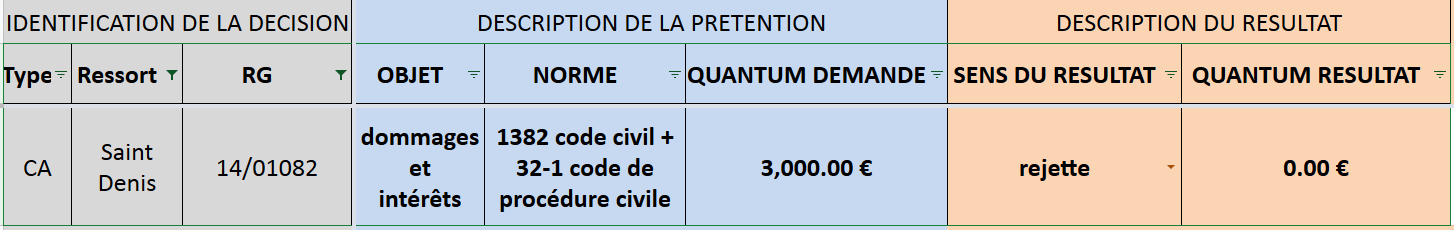
\includegraphics[width=0.8\textwidth]{tab-danais.png}
\end{exampleblock}

\begin{alertblock}{\scriptsize Difficultés}
	\begin{itemize}\scriptsize 
		\item Présence de plusieurs demandes de catégories similaires et/ou différentes dans une même décision
		\item Toutes les catégories ne sont pas connues d'avance (+500 catégories)
		\item Difficile d'annoter une base d'évaluation pour toutes les couvrir
	\end{itemize}
\end{alertblock}
\end{frame}

\subsection{Méthode : identifier les passages, puis les informations}

\begin{frame}[c]{Retrouver les demandes à l'aide des termes clés}
%	\begin{itemize}	\scriptsize
%		\item Phase d'entraînement	
%		\begin{itemize} \scriptsize
%			\item entraînement d'un classifieur pour détecter la présence d'une catégorie
%			\item Détermination automatique de la terminologie de la catégorie : 
%		\end{itemize}
%	\item Phase d'extraction
	\begin{enumerate} \scriptsize
		\item Identification de la catégorie par classification de textes 
		\item Exploiter la proximité entre \textbf{vocabulaire de la catégorie} et sommes d’argent pour extraire les quanta:
		
		Section Litige : identification de la demande
		
		\fbox{\parbox{0.8\textwidth}{\scriptsize
				Jennifer M. et Catherine M. ... demandent à la Cour de :
				
				- infirmer le dit jugement en toutes ses dispositions ; 
				...
				
				Statuant à nouveau ...
				
				- \textbf{[} les \underline{condamner} au paiement d' une somme de  \textit{$3 000,00$ €} \textbf{pour procédure abusive} et
				aux entiers dépens ; \textbf{]}$_\text{demande\_danais}$
				
				 ...							
		}}
	
	Section Dispositif : identification du résultat
	\fbox{\parbox{0.8\textwidth}{\scriptsize			
			La cour ... 
			
			CONFIRME le jugement entrepris en toutes ses dispositions.
	}}
		\item Lier les informations relatives à la même demande
	\end{enumerate}
	
%	\end{itemize}
\end{frame}
\subsection{Expérimentations sur 6 catégories de demandes}
\begin{frame}{Données}
	\begin{figure}[!htb]
		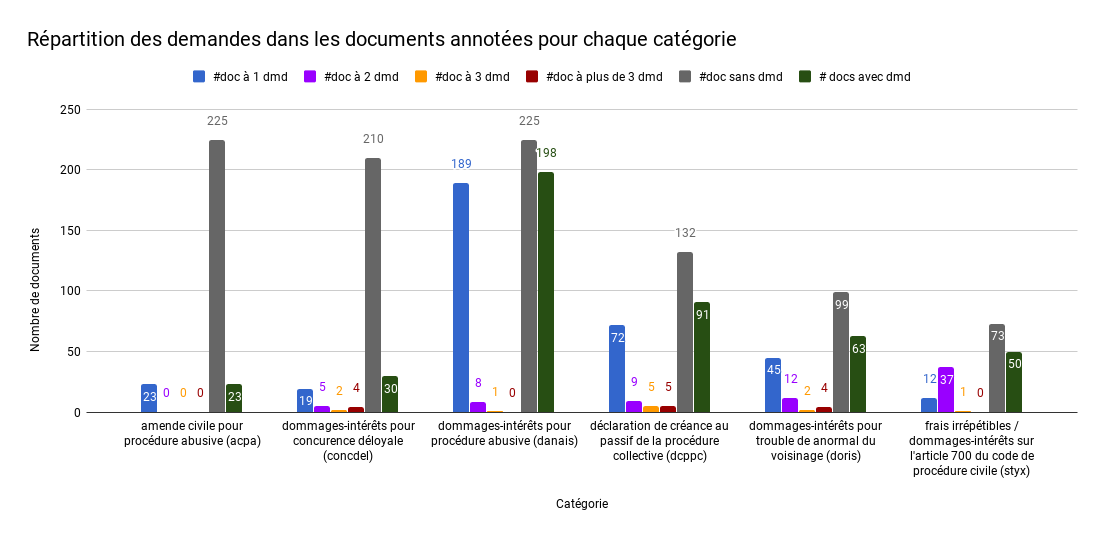
\includegraphics[width=0.8\textwidth]{chartDataset.png}
		\caption{\scriptsize Répartitions des demandes dans les documents annotées.}\label{fig:quanta:hist-repartition-docs}
	\end{figure}	
\end{frame}


\begin{frame}[c]{Résultat : Extraction}
	\begin{itemize} \small
		\item Détection de catégorie facile par des classifieurs traditionnels (K-plus-proches-voisins, SVM, Bayésien naïf, Arbre) : $98.8\% \leq$ F$_1$-mesure $\leq 100\%$
		\item Extraction des quantas et sens du résultat
			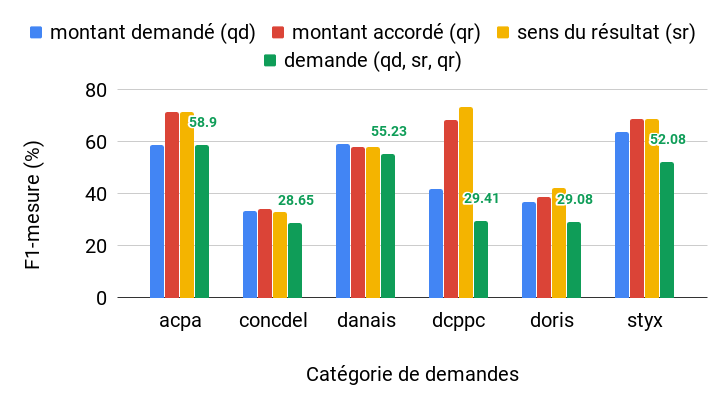
\includegraphics[width=0.9\textwidth]{f1-quanta-et-sens.png}
	\end{itemize}
\end{frame}
